A simulação para o modelo de \textit{trapping-detrapping} explicado na Seção \ref{sec:trap-detrap-plasma-cc} com concentração da superfície dada pela condição de nitretação por plasma, utilizou os parâmetros mencionados na Seção \ref{params_sub}, os parâmetros para nitretação à gás da Seção \ref{sec:param-plasma}, $H_{superficie}$=5,0$\times$ 10$^{23} m^{-2}$ (obtido pelo melhor \textit{fit}) temperatura de 673K e os seguinte valores para a aplicação do método numérico:$\Delta t$ e $\Delta x$ utilizados foram 0,0001s e 0,1 $\mu m$, para um tempo total de 2 horas e 20 $\mu m$ de profundidade.

As Figuras \ref{fig:td-csvar-plasma} e \ref{fig:td-csvar-plasma-both} mostram as solução da simulação após 2 horas de nitretação. Os resultados experimentais de \cite{moskalioviene2011modeling} não foram adicionados por conta da grande diferença nos valores, que tornariam o gráfico pouco informativo.

\begin{figure}[ht]
\centering
	\caption{Resultado simulação para o modelo de \textit{trapping-detrapping} para nitretação a plasma, até 2 horas}
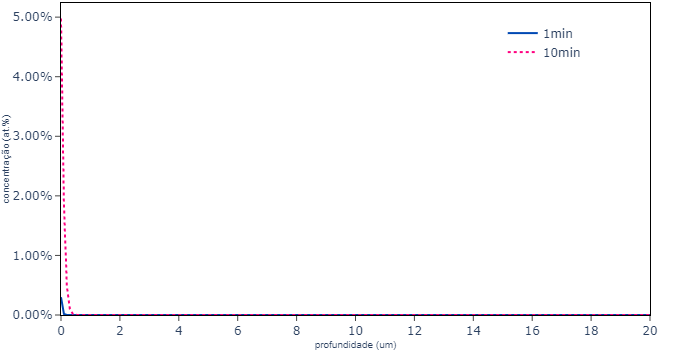
\includegraphics[width=1.0\textwidth]{plot_TrapDetrapPlasma}
	\label{fig:td-csvar-plasma}
	\centering
	\fonte{Elaborado pela autora}
\end{figure}

\begin{figure}[ht]
\centering
	\caption{Resultado simulação para o modelo de \textit{trapping-detrapping} para nitretação a plasma - Perfil de Concentração de nitrogênio Livre e Aprisionado, após 2 horas}
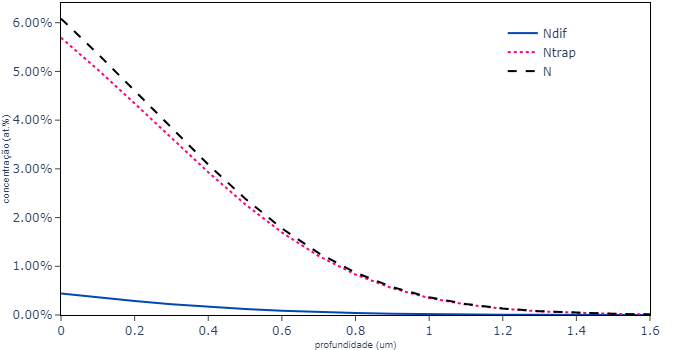
\includegraphics[width=1.0\textwidth]{plot_TrapDetrapPlasma2hBoth}
	\label{fig:td-csvar-plasma-both}
	\centering
	\fonte{Elaborado pela autora}
\end{figure}